% Options for packages loaded elsewhere
\PassOptionsToPackage{unicode}{hyperref}
\PassOptionsToPackage{hyphens}{url}
\documentclass{beamer}
\usepackage{graphicx}
\usepackage{amsmath}
\usepackage{booktabs}
\usepackage{xcolor}
\usepackage{bookmark}

% Penn colors
\definecolor{pennred}{HTML}{990000}
\definecolor{pennblue}{HTML}{011f5b}

% Beamer theme settings
\usetheme{Madrid}
\setbeamercolor{structure}{fg=pennred}
\setbeamercolor{frametitle}{bg=pennblue, fg=white}
\setbeamercolor{title}{fg=white}
\setbeamercolor{item}{fg=pennred}

\title[Beyond Expected Goals]{Beyond Expected Goals: A Probabilistic Framework for Shot Occurrences in Soccer}
\author[Feng, Pipping, and Sabin]{Tianshu Feng, Jonathan Pipping, and Paul Sabin}
\date{\today}
\institute[UPenn]{University of Pennsylvania}

\begin{document}

\frame{\titlepage}

% What Are Expected Goals (xG)?
\begin{frame}{What Are Expected Goals (xG)?}
\begin{itemize}
\item Expected Goals (xG) is a metric that estimates the probability that a shot is scored
\item Depends on factors like distance from goal, angle to goal, shot type, and player positions
\item Estimated by XGBoost models trained on historical shot data
\item Often used to measure the quality of a chance
\item Aggregated over a match or season to measure team performance
\end{itemize}
\end{frame}

% Limitations of xG
\begin{frame}{Limitations of xG}
\begin{itemize}
\item Models are only trained on \textbf{observed} shots, inducing significant selection bias
\item Skilled attackers who take more shots are over-represented
\item Threatening attacks with no recorded shots are omitted
\item Aggregating xG across a match double-counts rebound chances
\end{itemize}
\end{frame}

% Visual Examples
\begin{frame}{Example 1: No Shot Recorded}

\end{frame}

\begin{frame}{Example 2: Multiple Shots Taken}

\end{frame}

% Our Target Metric: xG+
\begin{frame}{Our Target Metric: xG+}
\begin{itemize}
\item A more complete picture of goal expectancy
  \begin{itemize}
  \item Accounts for high-threat attacks with no shots
  \item Does not double-count rebound chances
  \end{itemize}
\item At each frame, we calculate the probability of a goal:
\begin{align*}
\mathbb{P}(\text{goal scored}) &= \mathbb{P}(\text{goal scored} \mid \text{shot taken})\cdot\mathbb{P}(\text{shot taken}) \\
  &= \text{xG}\cdot\text{xShot}
\end{align*}
\item And then define xG+ for each possession as the probability a goal occurs:
\end{itemize}
$$\text{xG+} = 1 - (1 - \mathbb{P}(\text{goal scored})^{\text{n\_frames}})$$
\end{frame}

% Estimating xShot
\begin{frame}{Estimating xShot}
\begin{itemize}
\item \texttt{xShot}: the probability that a shot occurs in the next second
\item Build a model to estimate \texttt{xShot} based on features from tracking data
\item Also build our own version of \texttt{xG} model using the same features on observed shots
\end{itemize}
\end{frame}

% Data Processing
\begin{frame}{Data Processing}
\begin{itemize}
\item Remove games where no shots are recorded
\item Only keep frames where the ball is in play and a team has clear possession
\item Linearly interpolate ball positions to fill in missing frames
\item \texttt{attack}: Index of the attack the current frame is on (0 if it is not on an attack)
  \begin{itemize}
  \item Start with the attacking team gaining possession in their attacking third
  \item End with the defending team regaining possession or the ball is out of their attacking third
  \item Only keep frames with \texttt{attack} > 0
  \end{itemize}
\end{itemize}
\end{frame}

\begin{frame}{Data Processing}
\begin{itemize}
\item Rotate the coordinates $180^{\circ}$ around the center point for frames where the team attacks from right to left to unify the attacking directions and make all $x$-coordinates positive
\item Use a polar coordinate system centered on the goal for the ball
  \begin{itemize}
  \item $r_{ball}$ and $\theta_{ball}$ represent the distance and angle of the ball from the goal
  \item Keep the $z$-coordinate and compute the speed of the ball
  \end{itemize}
\item Use a polar coordinate system centered on the ball for each player
  \begin{itemize}
  \item Choose the 5 closest offense teammates and non-GK defenders to the ball as features
  \item Keep goalkeeper positions as a separate feature
  \end{itemize}
\end{itemize}
\end{frame}

\begin{frame}{Data Processing}
\begin{itemize}
\item \texttt{openGoal}: Percentage of the goal that is open from the ball's position
  \begin{itemize}
  \item Simplify every defender as a circle with a radius of 0.75 m
  \item Compute the two tangent lines from the ball to every defender in front of the ball their intersection points with the goal line
  \item Calculate the length of the open goal as the length of goal not covered by segments formed by the intersection points
  \end{itemize}
\end{itemize}
\end{frame}

% Model Specifications
\begin{frame}{Model Specifications}
\begin{itemize}
\item Trained on all tracking data of 2022-2025 Premier League seasons
\item Use a 5-fold cross-validation to evaluate both \texttt{xG} and \texttt{xShot} XGBoost models
\item Choose log loss as the evaluation metric
\end{itemize}
\end{frame}

% Results
\begin{frame}{Results}
\begin{columns}[c]
  \column{0.4\textwidth}
  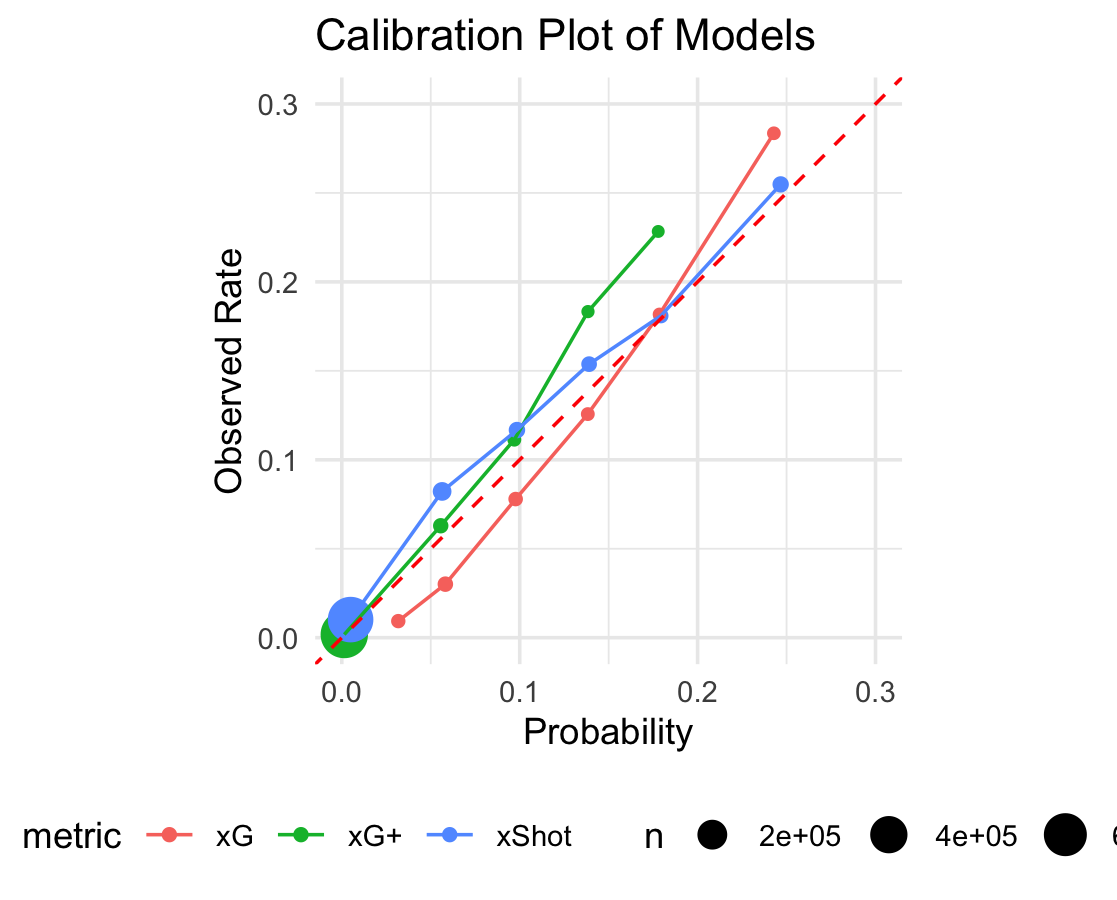
\includegraphics[width=\linewidth]{figures/calibration_1.png}
  
  \column{0.4\textwidth}
  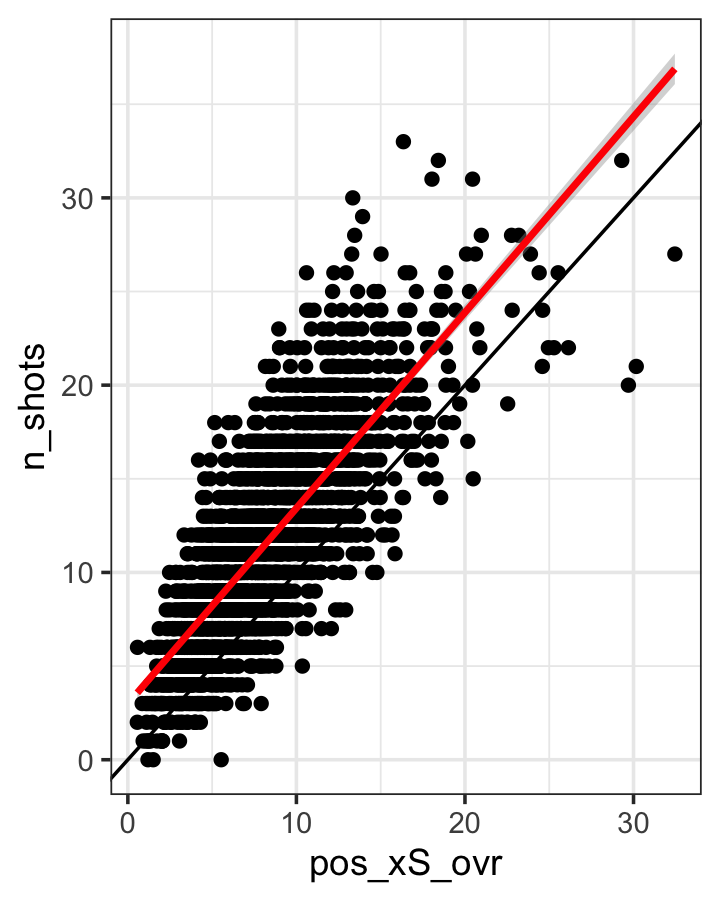
\includegraphics[width=\linewidth]{figures/calibration_2.png}
\end{columns}
\end{frame}

% Cross-Validation Study
\begin{frame}{Cross-Validation Study}
\begin{itemize}
\item \textbf{Objective}: Evaluate xG+ performance using cross-validated Poisson models
\item \textbf{Dataset}: 3 seasons of match data (114 folds total)
\item \textbf{Method}: Train on all matchdays except one, predict goals on held-out data
\item \textbf{Goal}: Determine how well adjusted xG+ explains actual goals scored
\end{itemize}
\end{frame}

% Cross-Validation Setup
\begin{frame}{Cross-Validation Setup}
\begin{itemize}
\item Each matchday treated as a fold: $38 \text{ matchdays} \times 3 = 114$ folds
\item For each fold:
  \begin{itemize}
  \item Train on all matchdays except one to acquire adjusted metrics
  \item Poisson regression on team goals using training data
  \item Predict goals scored on held-out matchday test data
  \end{itemize}
\end{itemize}
\end{frame}

% Metrics and Aggregation Methods
\begin{frame}{Metrics and Aggregation Methods}
\textbf{Metrics:}
\begin{itemize}
\item \textbf{xS}: Probability a player takes a shot in the next second
\item \textbf{xG}: Probability of a goal (given a shot)
\item \textbf{xG+}: xS $\times$ xG, probability of scoring in the next second
\end{itemize}

\textbf{Aggregation Methods:}
\begin{enumerate}
\item \textbf{Max-per-possession}: Take maximum 1-second prediction in each possession
\item \textbf{At-least-one-per-possession}: $1 - \prod (1 - p)$ across possession
\item \textbf{Sum-of-shots}: Traditional xG summed over actual shots
\end{enumerate}
\end{frame}

% Mixed Effects Modeling
\begin{frame}{Mixed Effects Modeling}
\textbf{Fitted on training data for each fold:}
$$\texttt{metric} \sim (1|\texttt{season}) + (1|\texttt{season:team}) + (1|\texttt{season:opp}) + \texttt{home}$$

\textbf{Extracted effects:}
\begin{itemize}
\item Team attack (per season)
\item Opponent defense (per season)
\item Season effect
\item Home field advantage
\end{itemize}
\end{frame}

% Secondary Poisson Model
\begin{frame}{Secondary Poisson Model}
\textbf{Train Poisson regression on adjusted metrics:}
$$\texttt{goals} \sim \texttt{home} + \texttt{season} + \texttt{team\_off} + \texttt{opp\_def}$$

\textbf{Purpose}: Assess predictive utility of each adjusted metric on actual goals
\end{frame}

% Cross-Validation Results
\begin{frame}{Cross-Validation Results}
\begin{table}[!h]
\centering
\caption{Mean Squared Error (MSE) by Metric and Aggregation Method}
\begin{tabular}[t]{lrrr}
\toprule
Aggregation Method & xG+ & xS & xG\\
\midrule
At-least-one-per-possession & 2.84 & 2.90 & 2.94\\
Max-per-possession & 2.84 & 2.87 & 2.91\\
Sum-of-shots &  &  & 2.90\\
\bottomrule
\end{tabular}
\end{table}
\end{frame}

\begin{frame}{Cross-Validation Results}
\begin{table}[!h]
\centering
\caption{Mean Absolute Error (MAE) by Metric and Aggregation Method}
\begin{tabular}[t]{lrrr}
\toprule
Aggregation Method & xG+ & xS & xG\\
\midrule
At-least-one-per-possession & 1.86 & 1.87 & 1.89\\
Max-per-possession & 1.86 & 1.86 & 1.89\\
Sum-of-shots &  &  & 1.87\\
\bottomrule
\end{tabular}
\end{table}
\end{frame}

% Conclusions
\begin{frame}{Conclusions}
\begin{itemize}
\item \textbf{xG+ performs best}: Lowest MSE and MAE across all aggregation methods
\item \textbf{At-least-one-per-possession} aggregation method shows strongest performance
\item \textbf{Future work}: Compare to actual shot-based xG, consider time-weighted xS
\item \textbf{Questions and discussion}
\end{itemize}
\end{frame}

% Acknowledgements
\begin{frame}{Acknowledgements}
\begin{itemize}
\item Special thanks to our data providers at PFF FC and the English Premier League.
\item All work supported by the Wharton Sports Analytics \& Business Initiative (WSABI) Summer Research Lab.
\end{itemize}
\end{frame}

\end{document}
